\section{Median Filtering}
We could probably compute the total difference in gray levels between the original and filtered images.
But I'm not sure if that's a useful metric or not.

Or we could create two new images showing the difference in gray level values between the original and filtered images.
But then again, judging the quality of the result of an image filter is highly subjective and depends on what one is looking for.

Figure~\ref{fig:2-2-1} shows the median filter of varying sizes applied to images with salt \& pepper noise added.
While Figure~\ref{fig:2-2-2} shows it applied to images with gaussian noise added.

\begin{figure}[h]
    \centering

    \begin{subfigure}{0.3\textwidth}
        
\includegraphics[width=0.9\textwidth]{../code/2_out/2-1_sp.png}
        \caption{No filter.}
        \label{fig:2-2-1:1}
    \end{subfigure}
    \begin{subfigure}{0.3\textwidth}
        
\includegraphics[width=0.9\textwidth]{../code/2_out/2-2_sp_3x3.png}
        \caption{3x3}
        \label{fig:2-2-1:2}
    \end{subfigure}

    \begin{subfigure}{0.3\textwidth}
        
\includegraphics[width=0.9\textwidth]{../code/2_out/2-2_sp_5x5.png}
        \caption{5x5}
        \label{fig:2-2-1:3}
    \end{subfigure}
    \begin{subfigure}{0.3\textwidth}
        
\includegraphics[width=0.9\textwidth]{../code/2_out/2-2_sp_9x9.png}
        \caption{9x9}
        \label{fig:2-2-1:4}
    \end{subfigure}

    \caption{Median filter of varying sizes applied to image with salt \& pepper noise.}
    \label{fig:2-2-1}
\end{figure}


\begin{figure}[h]
    \centering

    \begin{subfigure}{0.3\textwidth}
        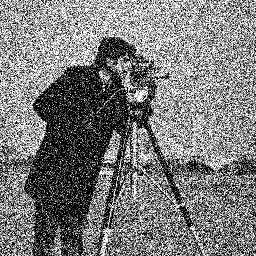
\includegraphics[width=0.9\textwidth]{../code/2_out/2-1_gaus.png}
        \caption{No filter.}
        \label{fig:2-2-2:1}
    \end{subfigure}
    \begin{subfigure}{0.3\textwidth}
        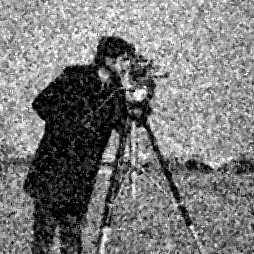
\includegraphics[width=0.9\textwidth]{../code/2_out/2-2_gaus_3x3.png}
        \caption{3x3}
        \label{fig:2-2-2:2}
    \end{subfigure}

    \begin{subfigure}{0.3\textwidth}
        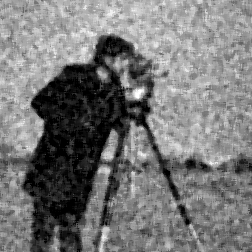
\includegraphics[width=0.9\textwidth]{../code/2_out/2-2_gaus_5x5.png}
        \caption{5x5}
        \label{fig:2-2-2:3}
    \end{subfigure}
    \begin{subfigure}{0.3\textwidth}
        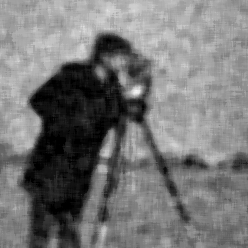
\includegraphics[width=0.9\textwidth]{../code/2_out/2-2_gaus_9x9.png}
        \caption{9x9}
        \label{fig:2-2-2:4}
    \end{subfigure}

    \caption{Median filter of varying sizes applied to image with gaussian noise.}
    \label{fig:2-2-2}
\end{figure}
